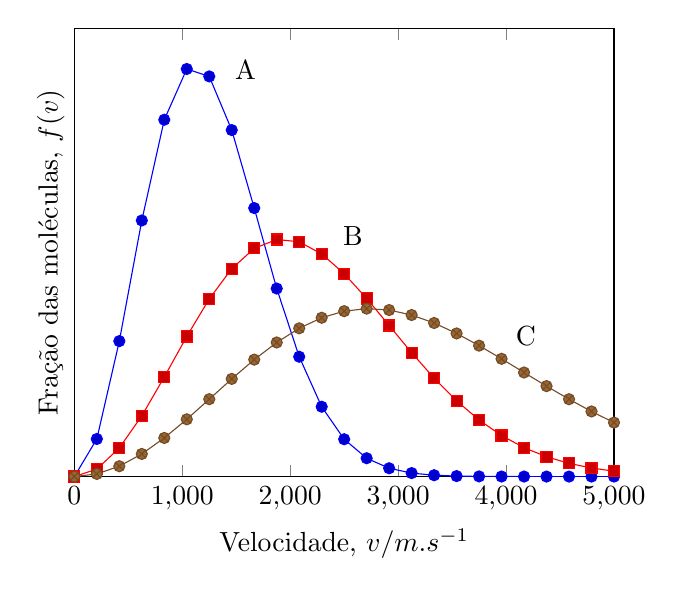
\begin{tikzpicture}
    \def\R{1000*8.314}% boltzmann constant
    \begin{axis}
        [
            grid = minor,
            domain = 0:5000,
            xlabel = {Velocidade, $v/\unit{m.s^{-1}}$},
            ylabel = {Fração das moléculas, $f(v)$},
            xmin=0, ymin=0,
            ytick = \empty,
            xmax=5000,
        ]
    \pgfplotsinvokeforeach{ 300, 900, 1800 }
        {
            \addplot
                {
                    sqrt(2/pi)*(4/(\R*#1))^(3/2)*x^2*exp(-4/(\R*#1)*x^2/2)
                };
        }

    \node [anchor = south west] at (axis cs:1400,0.0007) 
        { \ce{A} };
    \node [anchor = south west] at (axis cs:2400,0.0004) 
        { \ce{B} };
    \node [anchor = south west] at (axis cs:4000,0.00022) 
        { \ce{C} };
\end{axis}
\end{tikzpicture}
